%%%%%%%%%%%%
%
% $Autor: Wings $
% $Datum: 2019-03-05 08:03:15Z $
% $Pfad: Automatisierung/Skript/Produktspezifikation/Powerpoint/AMF.tex $
% $Version: 4250 $
%
%%%%%%%%%%%%



%todo Eigene Bilder
%todo https://ieeexplore.ieee.org/abstract/document/8100841 lena   - general\

\section{Images and Image Classification with a \ac{cnn}}


The classification of images is divided into two areas: image classification and object classification. 
Object classification attempts to identify one or more objects. The identification is done by assigning them to predefined classes. As a rule, the results are given with probabilities. Image classification attempts to identify a suitable description for the image; in this case, the image is recorded and interpreted in its entirety. \cite{Zhiqiang:2017}

Several challenges exist when classifying images. If one uses images, one is processing larger amount of data. An image with $200 \times 200$ pixels has 40,000 pixels. If it is a colour image with three colour channels, one processes 120,000 attributes. 
Furthermore, it is desirable that the result of the classification is independent of affine mappings. That is, the result is independent of scaling or rotation of the image. If only a section of the image is examined, the corresponding result should still be delivered. The mapping~\ref{img:challenges} represents an image with corresponding operations.  
The classic \glqq Lena\grqq{} of image processing is used as the basis of the demonstration \cite{Munson:1996}. This is an image of Lena Soderberg from 1972 that is available in the USC-SIPI Image Database \cite{Weber:1997}.



\begin{figure}[!h]
	%\begin{subfigure}[h]{0.4\linewidth}    
	%todo Eigene Bilder    
	\centering
	\begin{tabular}{cc}
		\includegraphics[width=0.4\textwidth]{Images/lena}    &
		\includegraphics[width=0.4\textwidth,trim=30 30 90 90,clip]{Images/lena}    \\
		\includegraphics[width=0.4\textwidth,angle=90]{Images/lena}    &
		\includegraphics[width=0.4\textwidth]{Images/lenaCrop}    \\
	\end{tabular}
	\caption{Original image, scaling, rotation and cropping of the image}\label{img:Herausforderungen}
\end{figure}



\subsection{Representation of Images}

For a computer programme, an image is a matrix of numbers. The type of matrix is determined by the resolution, the number of colours and the colour depth. The resolution is the pair of values of how many elements, called pixels, the matrix has in height and in width. A simple example is shown in the image~\ref{img:black and white}. The image has a resolution of 10 pixels in width and in height. The values can be either 0 or 1; in this illustration the value 0 represents the colour black, 0 the colour white.


\begin{figure}
	\begin{center}
		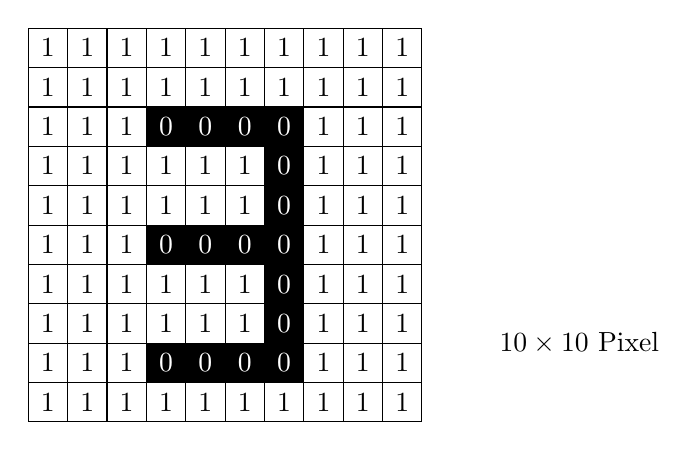
\begin{tikzpicture}
			
			%        \only<5->
			{
				\foreach \j in {0.5,1,...,5} 
				{
					\foreach \i in {0.5,1,...,5} {
						
						\node (P1) at (\i-0.25,\j-0.25) {1};
					}
				}
			}
			
			\draw[step=0.5,black,thin] (0,0) grid (5,5);
			
			%        \only<2->
			{
				
				\draw[fill=black] (1.5,0.5)  -- (2,0.5) -- (2,1) -- (1.5,1) -- cycle;
			}
			%        \only<3->
			{
				
				\draw[fill=black] (1.5,0.5)  -- (3.5,0.5) -- (3.5,1) -- (1.5,1) -- cycle;
				\draw[fill=black] (3,1)  -- (3.5,1) -- (3.5,4) -- (3,4) -- cycle;
				\draw[fill=black] (1.5,2)  -- (3.5,2) -- (3.5,2.5) -- (1.5,2.5) -- cycle;
				\draw[fill=black] (1.5,3.5)  -- (3.5,3.5) -- (3.5,4) -- (1.5,4) -- cycle;
			}
			
			%        \only<4->
			{
				\node (P1) at (1.75,0.75) {\textcolor{white}{0}};
				\node (P1) at (2.25,0.75) {\textcolor{white}{0}};
				\node (P1) at (2.75,0.75) {\textcolor{white}{0}};
				\node (P1) at (3.25,0.75) {\textcolor{white}{0}};
				\node (P1) at (3.25,1.25) {\textcolor{white}{0}};
				\node (P1) at (3.25,1.75) {\textcolor{white}{0}};
				\node (P1) at (3.25,2.25) {\textcolor{white}{0}};
				\node (P1) at (3.25,2.75) {\textcolor{white}{0}};
				\node (P1) at (3.25,3.25) {\textcolor{white}{0}};
				\node (P1) at (3.25,3.75) {\textcolor{white}{0}};
				
				\node (P1) at (1.75,2.25) {\textcolor{white}{0}};
				\node (P1) at (2.25,2.25) {\textcolor{white}{0}};
				\node (P1) at (2.75,2.25) {\textcolor{white}{0}};
				
				\node (P1) at (1.75,3.75) {\textcolor{white}{0}};
				\node (P1) at (2.25,3.75) {\textcolor{white}{0}};
				\node (P1) at (2.75,3.75) {\textcolor{white}{0}};
			}
			
			%        \only<6->
			{
				\node (Pixel) at (7,1) {$10 \times 10$ Pixel};
			}      
			
		\end{tikzpicture}
	\end{center}    
	
	
	\caption{Structure of a black and white image with $10 \times 10$ pixels}\label{img:schwarzweiss}
\end{figure}


Typical resolutions for camera images are recorded in the table\ref{image:resolution}. A pixel is defined by the number of colours and the colour depth. The colour depth indicates the range of values taken from the individual elements. These are usually integer values, specified in bits. Thus, an 8-bit value corresponds to a number between 0 and 255. A pixel can now contain such a numerical value for each colour. Often, however, a separate matrix is used for each colour. If one works with the RGB representation, one has the colours red, green and blue. The colour impression is obtained by superimposing the three images. The situation is shown in the figure~\ref{image:lenaRGB}. 



\begin{table}
	\centering
	\begin{tabular}{lcc}
		Resolution &=& width $\times$ height \\
		VGA             &=& $640 \times 480$ \\
		HD              &=& $1280 \times 720$\\
		Full HD         &=& $1920 \times 1080$\\
		4K               &=& $3840 \times 2160$\\
	\end{tabular}
	\caption{Standard resolutions of camera images}\label{Bild:Aufloesung}  	
\end{table}

\bigskip



\begin{figure}
	\centering
	\begin{tikzpicture}
		\node (P1) at (0,0) {\includegraphics[width=0.2\textwidth]{Images/LenaBlue}};
		\node (P1) at (2,0) {$+$};
		\node (P1) at (4,0) {\includegraphics[width=0.2\textwidth]{Images/LenaRed}};
		\node (P1) at (6,0) {$+$};
		\node (P1) at (8,0) {\includegraphics[width=0.2\textwidth]{Images/LenaGreen}};
		\node (P1) at (10,0) {$=$};
		\node (P1) at (12,0) {\includegraphics[width=0.2\textwidth]{Images/lena}};
	\end{tikzpicture}
	\caption{Image with 3 colour channels}\label{Bild:lenaRGB}
\end{figure}

Often greyscales are used instead of colour images. For this purpose, 256 greyscales are often used.% according to Figure~\ref{Image:256Greyscales}. 
When converting a colour image with three colours, the three matrices are added weighted. It has been shown that equal weighting of the colour channels is inappropriate. The OpenCV library for processing images uses the following weighting \cite{OpenCV:2020b}:

% Source: https://latexref.xyz/_005cincludegraphics.html
$$0.299 \cdot \hbox{Red} +0.587 \cdot \hbox{Green} +0.114 \cdot \hbox{Blue}$$

The conversion can be applied to the image \glqq Lena \grqq{}; this is in the figure~\ref{image:lenaGray}. Other weights are used depending on the application. 
The above weights are empirically determined and are proportional to the sensitivity of the human eye to each of the trichromatic colours. The image~\ref{image:lenaGray} has a colour depth of 8-bit. Other colour depths can also be used. A black and white image has the lowest colour depth. 

\begin{figure}[!h]
	\begin{center}
		
		%\begin{subfigure}[h]{0.4\linewidth}
		%todo Eigene Bilder    
		\includegraphics[width=0.7\textwidth]{Images/graylena}
		
		\caption{Greyscale with a value range from 0 to 255}\label{Bild:lenaGray}
	\end{center}    
\end{figure}




\begin{figure}[!h]
	\begin{center}
		
		%\begin{subfigure}[h]{0.4\linewidth}
		%todo Eigene Bilder    
		
		\includegraphics[width=0.3\textwidth]{Images/lenaBlackWhite126}
		\quad
		\includegraphics[width=0.3\textwidth]{Images/Grayscale4}
		\quad
		\includegraphics[width=0.3\textwidth]{Images/graylena}
		
		\caption{Black and white image, image with 4 grey levels and with 256 grey levels.}\label{Bild:}
	\end{center}    
\end{figure}


However, the quality of the image does not only depend on the parameters mentioned. The sharpness of the image also contributes to it. However, there is unfortunately no simple definition here, but is often shaped by subjective perception. On the other hand, it is possible to influence image sharpness by mathematical operations.  Blurring of an image can be achieved by blurring. 
Each pixel value is thereby represented by the average of the pixel values in a small window centred on the pixel. 

The resolution of the image affects the amount of computation required. For an image with a resolution of $674 \times 1200$ and a window size of $101 \times 101$, the new pixel value must be calculated separately for all three colour channels. In total this results in

$$674 \cdot 1200 \cdot 101 \approx 8.2 \cdot 10^9$$

operations. An example is shown in the figure~\ref{image:Blurring} with a filter size $5 \times 5$.


\begin{figure}
  \centering
  
  \includegraphics[width=0.3\textwidth]{Images/lenaBlurring}

  \caption{Softened image with a $5 \times 5$ filter}\label{Bild:Blurring}
\end{figure}


Another possibility of image processing is edge detection. With edge detection, the goal is to identify regions of the image where intensities of colour differ greatly. This is used to delineate objects and for object recognition. An example is given in Figure~\ref{image:edges}.

%
%Was ist ein Rand in einem Bild?
%Horizontaler Rand in Reihe i: Bild(i-1,j) unterscheidet sich stark
%von Bild(i+1,j)
%Vertikale Kante bei Spalte j: Bild(i,j-1) unterscheidet sich stark von
%Bild(i,j+1)
%Idee: Berechnen Sie für jede Position (i,j) und jede Farbe (RGB)
%change_hor = image(i-1,j, color) - image(i+1,j, color)
%change_vert = image(i,j-1, color) - image(i,j+1, color)
%edge_image(i,j,color) = sqrt( change_hor 2 + changevert 2 )
%

\begin{figure}
	\centering
	
	\includegraphics[width=0.3\textwidth]{Images/lenaBlackWhite}
	
	\caption{Edge detection on an image}\label{Bild:Kanten}
\end{figure}

%    \includegraphics[width=0.7\textwidth]{Images/lena}
%    \includegraphics[width=0.7\textwidth]{Images/rgbChannel}


%todo https://gist.github.com/MarcWang/b8e715200775079e4653


%\begin{figure}
%  \centering
%  \begin{tikzpicture}
%     \draw[\fill=left color=black!100!black,right color=white]  rectangle(0.7*\paperwidth,7mm);
%                
%                %            \fill[path fading=south,black!60!white](0,0)rectangle(\paperwidth,-0.1cm);
%                %            \node[text=white,anchor=west,text width=0.7\paperwidth, inner sep=0pt] at (0.03\paperwidth,1.5) {};
%        
%        
%        \node (P1) at (0,1) {0};
%        \node (P2) at (10,1) {255};
%        
%  \end{tikzpicture}
%  \caption{Balken mit 256 Graustufen}\label{Bild:256Grustufen}
%\end{figure}    

